\documentclass[12pt,a4paper]{article}
% Change "article" to "report" to get rid of page number on title page
\usepackage{amsmath,mathtools,amsfonts,amsthm,amssymb}
\usepackage{setspace}
\usepackage{Tabbing}
\usepackage{fancyhdr}
\usepackage{lastpage}
\usepackage{extramarks}
\usepackage{chngpage}
\usepackage{fourier}
\usepackage{soul,color}
\usepackage[usenames,dvipsnames]{xcolor}
\usepackage{graphicx,float,wrapfig}
\usepackage[utf8]{inputenc}
\usepackage{sidecap}
\usepackage{marvosym}
\usepackage{tikz, tikz-qtree}
\usepackage{tabularx, multirow}
\usepackage{enumerate}
\usepackage{hyperref}
\definecolor{gray99}{gray}{.99}
\usepackage{listings}
\usepackage[english]{babel}
\usepackage{placeins}
\usepackage{tikz}
\usepackage{tikz-qtree}
\usepackage{xspace}
\usepackage{mathtools}
\usepackage{tabulary}
\lstset{
	language=Caml,
	backgroundcolor=\color{gray99},
	tabsize=3,
	frame=single,
	keywordstyle=\ttfamily\bfseries\color{RoyalBlue},
	commentstyle=\ttfamily\color{ForestGreen},
	stringstyle=\ttfamily\color{Gray},
	breaklines=true,
	showstringspaces=false,
	basicstyle=\small\ttfamily,
	emph={label},
	xleftmargin=22pt,
	framexleftmargin=22pt,
	framexrightmargin=0pt,
	framexbottommargin=4pt,
	numbers=left,
	stepnumber=1
}
\usepackage{caption}
\DeclareCaptionFont{black}{\color{black}}{\bfseries}
\DeclareCaptionFormat{listing}{\parbox{\textwidth}{\hspace{8pt}#1#2#3}}
\captionsetup[lstlisting]{format=listing,labelfont=black,textfont=black, singlelinecheck=false, margin=0pt, font={bf,footnotesize}}

% In case you need to adjust margins:
\topmargin=-0.45in      %
\evensidemargin=0in     %
\oddsidemargin=0in      %
\textwidth=6.5in        %
\textheight=9.5in       %
\headsep=0.25in         %

% Special font
\newcommand{\cps}[2]{\ensuremath{[[{#1}]]_{\textstyle #2}}}

% Homework Specific Information
\newcommand{\hmwkTopic}{Data representation}
\newcommand{\hmwkTitle}{HW1 - \hmwkTopic}
\newcommand{\hmwkDueDate}{February 10, 2014}
\newcommand{\hmwkClass}{CS 199}
\newcommand{\hmwkAuthorNameA}{Sam Laane}
\newcommand{\hmwkAuthorEmailA}{laane2@illinois.edu}
\newcommand{\hmwkAuthorNameB}{José Vicente Ruiz}
\newcommand{\hmwkAuthorEmailB}{ruizcep2@illinois.edu}

% Setup the header and footer
\pagestyle{fancy}                                                       %
\lhead{\hmwkAuthorNameA \xspace \& \hmwkAuthorNameB}                                                 %
\chead{\hmwkClass}  %
\rhead{\hmwkTopic}     
                                                %
\lfoot{}                                                      %
\cfoot{\thepage}                                                        %
\rfoot{}                          %
\renewcommand\headrulewidth{0.4pt}                                      %
\renewcommand\footrulewidth{0.4pt}                                      %


%%%%%%%%%%%%%%%%%%%%%%%%%%%%%%%%%%%%%%%%%%%%%%%%%%%%%%%%%%%%%
% Make title
\title{\vspace{2in}\textmd{\hmwkClass\\\textbf{\hmwkTitle}}\\\normalsize\vspace{0.1in}\small{\hmwkDueDate}\\\vspace{4in}}
\date{}
\author{\textbf{\hmwkAuthorNameA} $\;$<\texttt{\href{mailto:laane2@illinois.edu}{\hmwkAuthorEmailA}}>\\\textbf{\hmwkAuthorNameB} $\;$<\texttt{\href{mailto:ruizcep2@illinois.edu}{\hmwkAuthorEmailB}}>}
%%%%%%%%%%%%%%%%%%%%%%%%%%%%%%%%%%%%%%%%%%%%%%%%%%%%%%%%%%%%%

\begin{document}
\begin{singlespace}

\begin{titlepage}
\maketitle
\thispagestyle{empty}
\end{titlepage}

% Uncomment the \tableofcontents and \newpage lines to get a Contents page
% Uncomment the \setcounter line as well if you do NOT want subsections
%       listed in Contents
%\setcounter{tocdepth}{1}
%\tableofcontents
\newpage

% When problems are long, it may be desirable to put a \newpage or a
% \clearpage before each homeworkProblem environment

\clearpage

\section{Dataset}

The dataset that we have chosen is about the red wine variant of the Portuguese ``Vinho Verde". The number of instances is 1599 and the available features of each of them are the following:

\begin{itemize}
    \item \textbf{Input variables} (based on physicochemical tests): 
    \begin{enumerate}
        \item fixed acidity 
        \item volatile acidity 
        \item citric acid 
        \item residual sugar 
        \item chlorides 
        \item free sulfur dioxide 
        \item total sulfur dioxide 
        \item density 
        \item pH 
        \item sulphates 
        \item alcohol 
    \end{enumerate}
    
    \item \textbf{Output variable} (based on sensory data): 
    \begin{enumerate}
        \setcounter{enumi}{11}
        \item quality (score between 0 and 10)
    \end{enumerate}
\end{itemize}

So our goal was to finger out what input variables determine the quality of a ``good'' red wine. Since we don't have details about the scoring process, we can just trust that is reliable. \\

In the beginning, we compared the remaining sugar with respect to the alcohol, however it proved useless. We have omitted the figure since it lacks of interest.

\newpage
\section{Histogram - Fixed acidity and Quality}

\begin{figure}[h!]
	\hspace{-1cm}
    \centering
    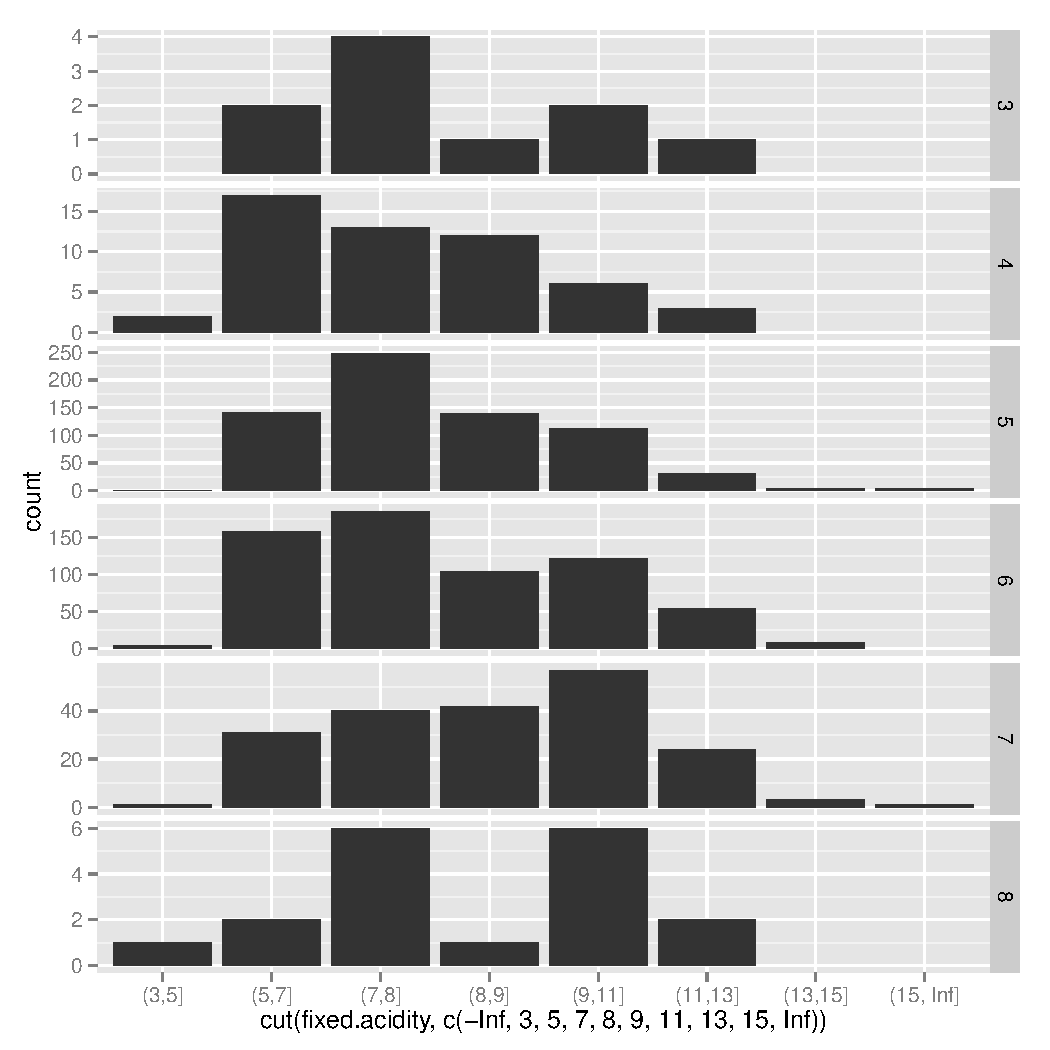
\includegraphics[width=\textwidth, height=19cm, trim= 0 0 0 20]{acidVSqual.pdf}
\end{figure}
\FloatBarrier
Another thing we have looked into was how the acidity affects the quality. 
While the over all trend seems to be that acidity does not matter that much we do observe
that the highest quality wine has a slightly higher or lower acidity score. 
It looks like people want a little excitement and find the the 8-9 range boring 
but don't want there red wines too strong.

\newpage
\section{Scatterplot - Alcohol, Density and Quality}

\begin{figure}[h!]
	\hspace{-1cm}
    \centering
    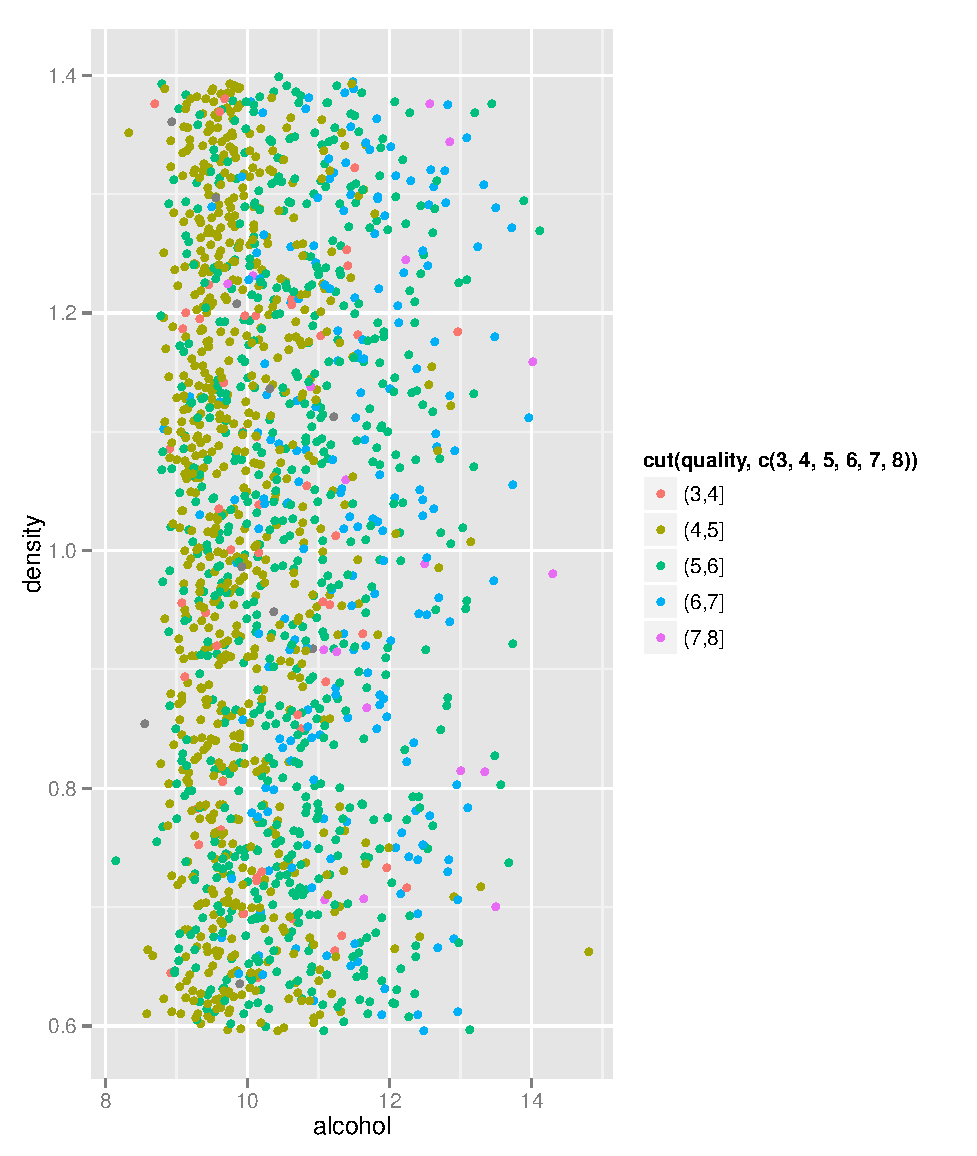
\includegraphics[width=\textwidth, height=19cm, trim= 0 0 0 20]{alcoholVSdensity.pdf}
\end{figure}
\FloatBarrier
It looks like density does not matter much in terms of alcohol content or quality. 
Wines have a large but even distribution of densities that have no correlation. 
Alcohol, however, seems quite interesting. Most wines seem to fall on the lower end of the alcohol scale. However, the few that have highest amounts of alcohol seem to have a higher quality.

\newpage
\section{Histogram - Alcohol and Quality}

\begin{figure}[h!]
	\hspace{-1cm}
    \centering
    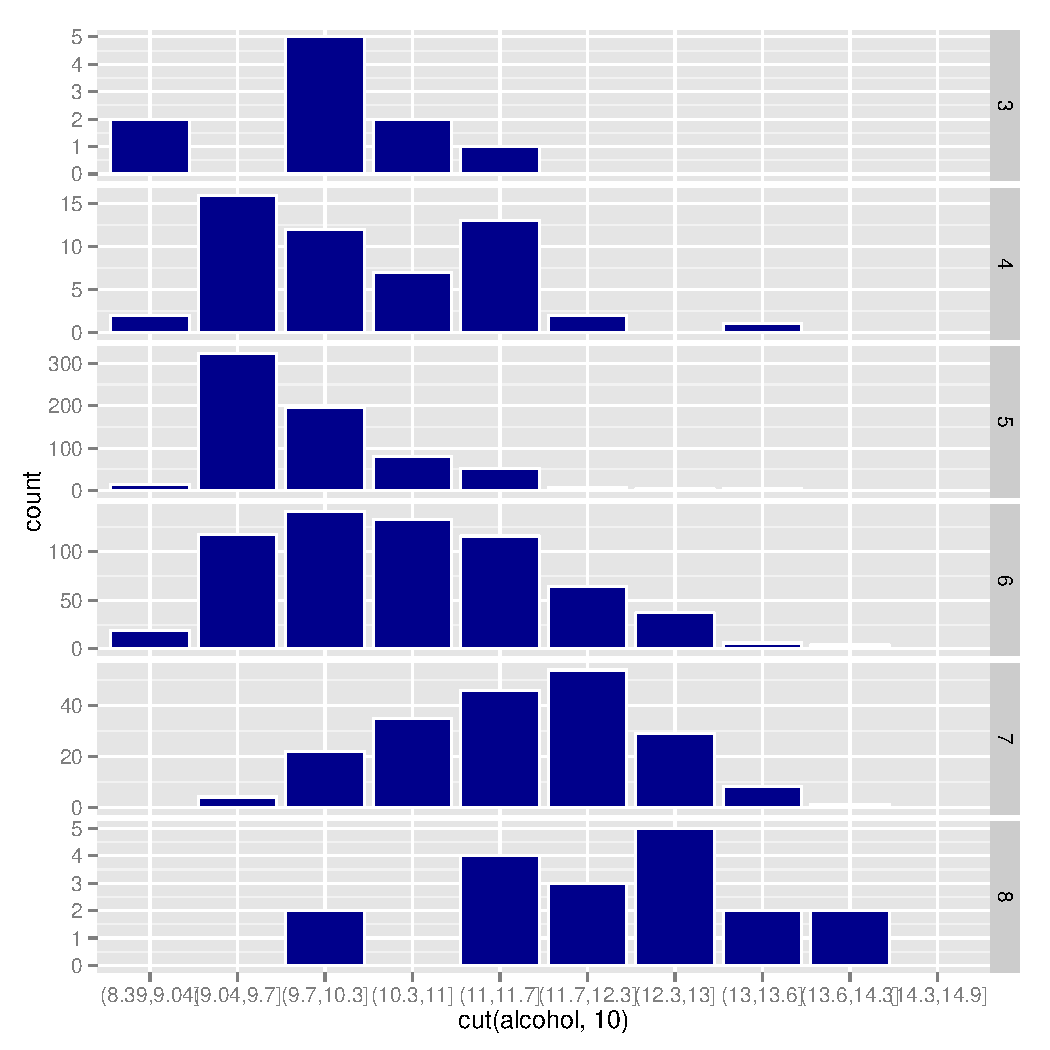
\includegraphics[width=\textwidth,trim= 0 0 0 20]{alcoholVSqual(blue).pdf}
\end{figure}
\FloatBarrier
The problem with our scatter plot was that, though we could see the thin distribution of high alcohol wines were seen as good, it was hard to tell whether or not the spread of good wines was also present under the large amounts of low quality, low alcohol wines. \\

This bar chart clearly shows that this is not the case. The best wines all seem to have larger amounts of alcohol. I would like to know why alcohol is the sole variable with such an impact. Could it be that the more alcohol the drinkers consumed the more they over looked the wines flaws? Or was it that quality was measured in an economic sense such that the more expensive the vino were said to be higher quality? Maybe people just like the test of alcohol. Whatever the reason it is clean that if one wanted to make a quality red they should focus on alcohol content.

\end{singlespace}
\end{document}
